\documentclass[11pt]{article}

% ---- arXiv-friendly preamble ----
\usepackage[margin=1in]{geometry}
\usepackage[T1]{fontenc}
\usepackage{lmodern}
\usepackage{microtype}
\usepackage{amsmath,amssymb}
\usepackage{booktabs}
\usepackage{graphicx}
\usepackage{xcolor}
\usepackage{tikz}
\usetikzlibrary{arrows.meta,positioning}
\usepackage[numbers,sort&compress]{natbib}
\usepackage[colorlinks=true,linkcolor=blue!60!black,citecolor=blue!60!black,urlcolor=blue!60!black]{hyperref}
\usepackage{enumitem}
\setlist{itemsep=2pt,topsep=3pt}
\emergencystretch=2em

% Unresolved-item markers. Every number in this draft is sourced from the
% netherite repository (docs/ARTICLE.md, docs/LAUNCH_POST.md, docs/GATES.md,
% docs/SCOPE.md, docs/CENSUS.md, magma/VERIFY.md, blaze/SPEC.md,
% verify/README.md, docs/DEVLOG.md); anything unmeasured is marked \todo.
\newcommand{\todo}[1]{\textcolor{red}{[TODO: #1]}}
\newcommand{\todoref}[1]{\textcolor{red}{[TODO: #1]}}

\title{\textbf{netherite}: A Bit-Verified C/CUDA Reimplementation of Minecraft\\for Large-Batch GPU Reinforcement Learning}

\author{Elliot Arledge\\
Independent Researcher\\
\texttt{elliot@arledge.net}\\
\url{https://github.com/Infatoshi/netherite}}

\date{}

\begin{document}
\maketitle

\begin{abstract}
Minecraft is arguably the best open-world reinforcement-learning benchmark in existence: procedurally infinite, long-horizon, hierarchical, and partially observable, with an enormous human prior. It is also a single-threaded Java client that advances one world at 20 ticks per second, so practitioners either train against the real game slowly or train in a Minecraft-\emph{like} substitute and absorb an unquantified sim-to-real gap. We present \textbf{netherite}, a from-scratch C/CUDA reimplementation of Minecraft 1.11.2 whose central contribution is not the engine but the \emph{verifier}: an oracle harness that instruments the real Java client to record tapes (inputs, per-tick physics state, entity streams, world snapshots, and lossless golden frames), then replays them tick-exact through the C engine behind frozen pass/fail gates. In the pinned 48-tape snapshot, 46 tapes are physics-clean at a $10^{-9}$ tolerance and 42 return pixel-gate rc~0; five of the six pixel failures remain within committed baselines, while one deliberately unabsorbed frame adds 2{,}409 pixels. On top of the verified core, a batched environment with a raycast semantic camera sustains 1.70M env-ticks/s (426{,}108 agent decisions/s) at batch 2{,}048 on an RTX~4090 and 1.62M env-ticks/s (405{,}998 decisions/s) on an RTX~5090, all measured at one pinned commit with machine-readable receipts. The project ships no Mojang content: users regenerate all assets locally from a legally owned copy of the game.
\end{abstract}

\section{Introduction}
\label{sec:intro}

Reinforcement learning in Minecraft has always faced a forced choice. The real game is faithful by definition but is a Java client that simulates one world at 20 ticks per second; platforms that wrap it, such as Malmo~\citep{johnson2016malmo}, MineRL~\citep{guss2019minerl}, and MineDojo~\citep{fan2022minedojo}, inherit that throughput ceiling. GPU-resident environments such as Isaac Gym~\citep{makoviychuk2021isaacgym}, Madrona~\citep{shacklett2023madrona}, and Craftax~\citep{matthews2024craftax} demonstrate that batched simulation can deliver orders of magnitude more experience per device, but for Minecraft specifically the fast options are Minecraft-\emph{likes}: Crafter~\citep{hafner2022crafter} and Craftax reproduce the game's \emph{spirit}, not its mechanics, and are not designed for direct policy transfer to the Java game.

netherite's bet is that the choice is false: make the substitute mechanically testable against the reference, then measure the remaining sim-to-real gap instead of assuming it away. Train in the reimplementation and evaluate the same frozen policy in both environments; paired failures become evidence for the next verifier or engine fix.

That bet only pays if exactness can be tested, and this paper's central claim is methodological: for a project of this shape, \textbf{the bottleneck is not the engine, it is the verifier}. Two prior attempts by the author died of exactly this disease (Section~\ref{sec:graveyard}): a clean-room Rust rewrite that could not even enumerate its divergences from the reference, and a pure-CUDA megakernel that was unbisectable when a long-running world diverged. The third attempt inverted the build order---the oracle came first---and is the system described here.

Concretely, netherite contributes:

\begin{enumerate}
\item \textbf{An oracle-based bit-verification methodology} (Section~\ref{sec:design}). The real 1.11.2 client runs with a small instrumentation mod that records \emph{tapes}: every input, every tick's post-tick player state at full float precision, the surrounding entity stream, a full world snapshot, and lossless golden frames at up to every tick. Replay drives the C engine tick-by-tick with the recorded inputs and fires frozen gates: physics (tolerance $10^{-9}$), state (inventory, health, world edits, entity counts), pixels (rendered frames vs.\ golden frames, clustered and classified with per-class budgets), and geometry (per-part transforms of articulated mobs). Every divergence that survives is filed in a public adversarial ledger with the tape, the tick, the pixel count, and the suspected mechanism.
\item \textbf{A verified engine with two explicit fidelity tiers} (Sections~\ref{sec:design}--\ref{sec:impl}). \texttt{magma}, the replay/playable tier, targets the real game: seed-derived worldgen, physics checked at $10^{-9}$ over recorded sessions, and a software rasterizer gated pixel-by-pixel against real-client screenshots, with CPU$=$CUDA parity gates including the depth buffer. \texttt{blaze}, the batched simulation tier, holds a different but equally mechanical contract: the CPU scalar path and the CUDA batch path are compiled from the same source and must agree bitwise on every tick.
\item \textbf{A batched GPU world architecture} (Section~\ref{sec:batched}) that keeps thousands of full Minecraft worlds resident in VRAM via palette-compressed chunk sections and an edit journal, uses stateless hash-based runtime RNG so parallel ticking is schedule-independent, and deliberately rejects the megakernel design in favor of small per-op kernels with scalar CPU twins.
\item \textbf{A pure-GPU semantic observation space} (Section~\ref{sec:camera}): training mode does not render at all. Each environment raycasts a $64\times36$ semantic camera (block ids, depth, edge flags) directly from world state---8{,}192 environments $\times$ 2{,}304 rays $\approx$ 19M rays per observation batch.
\item \textbf{Measured results} (Section~\ref{sec:eval}): exact-pin throughput receipts from two GPU generations; a pinned 48-tape verification suite with 42 pixel-gate rc~0 replays and one deliberately visible baseline regression; and a paired protocol that evaluates one frozen policy in both the simulator and the live Java client on identical seeds.
\end{enumerate}

netherite ships no Mojang content. The repository contains only original C/CUDA code and the harness; assets and reference behavior are regenerated locally from a copy of the game the user legally owns.

\section{Related Work}
\label{sec:related}

\paragraph{GPU-resident and large-batch RL environments.}
Isaac Gym~\citep{makoviychuk2021isaacgym} established the pattern of keeping both physics state and observations resident on the GPU, eliminating the CPU--GPU round trip that dominates conventional vectorized simulation; Brax~\citep{freeman2021brax} did the same in JAX for differentiable rigid-body physics. Madrona~\citep{shacklett2023madrona} generalizes the batch-world pattern into an ECS framework for many-world simulation, and EnvPool~\citep{weng2022envpool} attacks the same throughput problem on the CPU side with a highly parallel C++ execution engine. PufferLib~\citep{suarez2024pufferlib} focuses on making such environments interoperate cleanly with RL libraries at high throughput. netherite belongs to this family architecturally---worlds share nothing, state lives in VRAM, the host only exchanges action and observation tensors---but differs in target: the environment is not a purpose-built game or a physics scene, it is a bit-verified reimplementation of an existing commercial game.

\paragraph{Minecraft-likes built for RL throughput.}
Crafter~\citep{hafner2022crafter} distills Minecraft's achievement structure into a 2D benchmark; Craftax~\citep{matthews2024craftax} reimplements and extends it in JAX, delivering GPU-batched throughput that makes billion-step open-ended RL runs practical on a single device. These systems are deliberately \emph{inspired by} Minecraft rather than equal to it: their value is fast iteration on open-ended RL algorithms, and policies trained in them make no claim about the real game. netherite takes the complementary point in the design space: vanilla 1.11.2 mechanics, verified against the reference implementation, at batched-GPU throughput.

\paragraph{RL platforms on the real Minecraft.}
Malmo~\citep{johnson2016malmo} instruments the Java client for AI experimentation and is the ancestor of netherite's own oracle harness (the recorder mod is built on a Forge+Malmo client). MineRL~\citep{guss2019minerl} added large-scale human demonstrations and sample-efficiency competitions; MineDojo~\citep{fan2022minedojo} scaled task specification with internet knowledge; VPT~\citep{baker2022vpt} showed that behavioral priors pretrained from unlabeled video can reach long-horizon goals such as diamond tools; DreamerV3~\citep{hafner2023dreamerv3} learned to collect diamonds from scratch through a world model. All of these run the real Java game in the loop and therefore pay its per-world simulation cost. netherite's oracle harness runs the same Java client, but only to \emph{record and verify}; training never touches the JVM.

\paragraph{Positioning.}
To our knowledge, netherite is the first system to combine (i) a reimplementation of an existing game verified \emph{bitwise or pixelwise} against the shipped reference over recorded play, and (ii) large-batch GPU-resident RL on that verified core. The verification methodology (Section~\ref{sec:design}) is the transferable artifact: it applies to any ``rewrite the reference, but faster'' project, not just games.

\section{Design: The Verifier Is the Product}
\label{sec:design}

\subsection{Why oracle-first: a graveyard of two attempts}
\label{sec:graveyard}

This is the author's third serious run at this project, and the design is best motivated by why the first two died.

\textbf{Attempt 1: a clean-room Rust rewrite.} A working prototype reached the point where ``looks like Minecraft'' and ``is Minecraft'' had quietly diverged across mob pathing, item physics, and chunk decoration order, with no instrument that could enumerate the differences or drive them to zero. The code was fine; the epistemology was broken.

\textbf{Attempt 2: a pure-CUDA megakernel.} The entire game tick fused into one giant kernel over thousands of worlds, no CPU in the loop. The GPU part was fine. The problem was that a megakernel is a black box: when one world diverges from vanilla tens of thousands of ticks in, there is no per-subsystem seam to bisect against, no scalar reference to diff, no way to localize \emph{where} inside the fused tick it went wrong. Debugging correctness through a megakernel is archaeology.

Both attempts failed on verification, not simulation. There is also an uncomfortable scoping problem that no up-front test plan survives: which of the game's hundreds of blocks, items, and mobs are in scope, and how do you know the ones that are in actually behave under the weird, exploitable conditions real gameplay produces? Elytra wings through a waterfall; a blaze's aggro flag driving its fire engulfment; a nether portal entered four ticks after a recording started. These cases are discovered by playing, recording, and diffing---so the third attempt built the recorder before the engine.

\subsection{Two explicit fidelity contracts}
\label{sec:contracts}

netherite holds two different, mechanically checkable definitions of ``correct,'' and never conflates them:

\begin{itemize}
\item \textbf{Replay tier (\texttt{magma}): vanilla-exact on tape.} Given a recorded oracle session, the C engine must reproduce the recorded trajectory (positions and velocities to $10^{-9}$; health to $10^{-4}$; food and ground contact exactly), the recorded world edits and inventory, and---through its own software rasterizer---the recorded pixels, frame by frame, under frozen per-class budgets. The Java 48-bit worldgen LCG is replicated exactly; population that depends on vanilla chunk-load order is carried by the recorded world snapshot rather than claimed seed-exact.
\item \textbf{Batched tier (\texttt{blaze}): internal consistency.} The CPU scalar path and the CUDA batch path compile from the same \texttt{\_\_host\_\_ \_\_device\_\_} source and must agree \emph{bitwise} on every tick of every environment. This tier does not promise vanilla RNG call order or JVM float bit patterns---the three things (Java LCG call order, HashMap iteration order, \texttt{strictfp} bit patterns) whose pursuit killed the prior full-fidelity rewrites---but its behavior is anchored to the replay tier, which \emph{is} vanilla-checked, through shared physics code and shared gates.
\end{itemize}

\subsection{The oracle: making the real game testify}
\label{sec:oracle}

The real 1.11.2 client runs with a small instrumentation mod (\texttt{qrl}, built on a Forge+Malmo client). It can:

\begin{itemize}
\item record a \textbf{tape}: every input; every tick's post-tick player state (position and velocity at full float precision, health, food, fall distance, air, XP, potion effects, attack cooldown, hurt timers); the entity stream around the player (poses, health, hurt/death timers, status flags, item stacks); a whole-save world snapshot at recording start; inventory delta dumps on change; and \textbf{golden frames}---lossless screenshots at a fixed cadence, up to every tick, re-rendered at the tick boundary (\texttt{partialTicks}$=1.0$) so moving and static cameras are equally ground truth;
\item answer state queries over a socket---the same channel scripted scenarios use to stage worlds (fill blocks, summon mobs, hop dimensions);
\item write session facts into the tape header that replay cannot derive: the fog smoother's state at recording start, rain strength, which HUD overlays the capture stripped, and the full launch configuration (every option verbatim, plus the git revision), so a tape is only valid evidence when its sidecar matches the configuration under debug.
\end{itemize}

Replay drives the C engine tick-by-tick with the recorded inputs. Then the gates fire:

\begin{itemize}
\item \textbf{Physics gate}: the replayed trajectory must match the recorded one. Tolerance is $10^{-9}$ for positions and velocities (Minecraft physics is double-precision exact; anything larger is a real bug), exact for ground contact and food, $10^{-4}$ for health. The report names the \emph{first divergent tick and field}, which becomes the next bug.
\item \textbf{State gate}: inventory, health, world edits, entity counts.
\item \textbf{Pixel gate}: rendered frames vs.\ golden frames. Diff pixels are clustered and classified into accepted classes (HUD, viewmodel, particles, transit, \ldots) with per-class budgets; any \emph{unexplained} cluster of $\geq$4k pixels, or 8k unexplained pixels in a frame, fails the tape. A dedicated diff inspector names the \emph{cause} of each cluster (texel selection, shading offset, registration, cutout-sky, content, edge) rather than just its size, and re-derives its own verdicts from synthetic mutations on demand.
\item \textbf{Geometry gate}: for articulated mobs, the recorder dumps per-part transforms and the replay must reproduce them numerically (pass threshold 3.5 texels / 0.05\,rad after ring warmup). The gate emits an independently checkable receipt rather than relying on visual similarity.
\end{itemize}

Figure~\ref{fig:pipeline} summarizes the two evidence loops. The upper lane turns the shipped Java client into replayable ground truth; the lower lane keeps the high-throughput CPU and CUDA implementations bitwise coupled, then returns the learned policy to the Java client for the sim-to-real test.

\begin{figure*}[t]
\centering
\resizebox{\textwidth}{!}{%
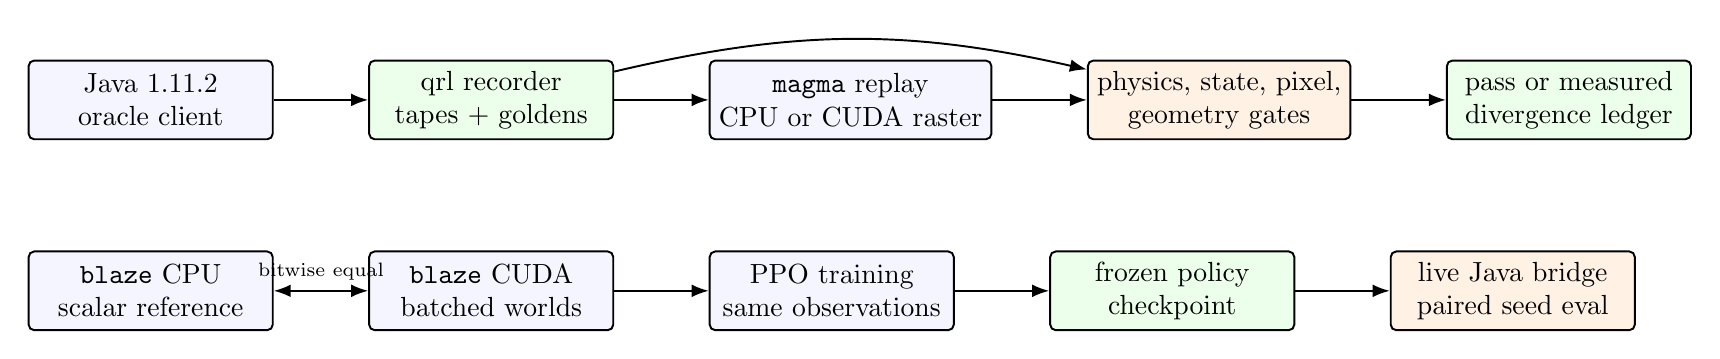
\begin{tikzpicture}[
  >=Latex,
  node distance=10mm and 12mm,
  box/.style={draw, rounded corners=2pt, align=center, minimum height=10mm,
              minimum width=31mm, fill=blue!4},
  gate/.style={box, fill=orange!10},
  evidence/.style={box, fill=green!8},
  every path/.style={draw, line width=0.7pt}
]
\node[box] (java) {Java 1.11.2\\oracle client};
\node[evidence, right=of java] (rec) {qrl recorder\\tapes + goldens};
\node[box, right=of rec] (magma) {\texttt{magma} replay\\CPU or CUDA raster};
\node[gate, right=of magma] (gates) {physics, state, pixel,\\geometry gates};
\node[evidence, right=of gates] (ledger) {pass or measured\\divergence ledger};

\node[box, below=14mm of java] (cpu) {\texttt{blaze} CPU\\scalar reference};
\node[box, right=of cpu] (cuda) {\texttt{blaze} CUDA\\batched worlds};
\node[box, right=of cuda] (ppo) {PPO training\\same observations};
\node[evidence, right=of ppo] (policy) {frozen policy\\checkpoint};
\node[gate, right=of policy] (real) {live Java bridge\\paired seed eval};

\path[->] (java) -- (rec);
\path[->] (rec) -- (magma);
\path[->] (magma) -- (gates);
\path[->] (rec) to[bend left=13] (gates);
\path[->] (gates) -- (ledger);
\path[<->] (cpu) -- node[above, font=\scriptsize] {bitwise equal} (cuda);
\path[->] (cuda) -- (ppo);
\path[->] (ppo) -- (policy);
\path[->] (policy) -- (real);
\end{tikzpicture}%
}
\caption{Verification and learning architecture. Tapes connect the real Java client to \texttt{magma}'s frozen fidelity gates; shared single-source simulation code connects the \texttt{blaze} scalar and CUDA paths. Policy transfer is evaluated by sending sampled policy actions back through the live Java bridge, not by replaying a seed or an action tape.}
\label{fig:pipeline}
\end{figure*}

The suite covers scenario families recorded from real play and from scripted scenarios: combat (blaze bow fights, melee, wither skeletons, pigman aggro), traversal (elytra through a waterfall and over lava, soul sand and ice, cobwebs, fence collisions), fluids (diving, flowing-water conversion), dimension transits (nether portal roundtrip, entering the End), the ender dragon fight, and long free-play sessions. A nightly sweep can replay every canonical tape on either backend and diffs every gate against committed baselines.

\subsection{The adversarial ledger}
\label{sec:ledger}

Everything that does not pass is filed in \texttt{OPEN\_DIVERGENCES.md}: the tape, the tick, the pixel count, the suspected mechanism, and often the vanilla source line. Closed entries retain full forensics in a companion ledger. Gate thresholds and divergence classes are frozen---a ``pass'' achieved by retuning is a lie, and the delegate acceptance script enforces this mechanically. Two consequences of taking the ledger seriously:

\begin{itemize}
\item \textbf{The oracle itself can be wrong.} netherite's fog never matched at the horizon; investigation eventually landed on the capture path rather than the rasterizer. Captures exhibit an approximately $1.05\times$ fitted radial-fog warp relative to the formula in Minecraft's source. llvmpipe is the leading mechanism, but remains a hypothesis pending a minimal reproduction; netherite therefore records the deviation rather than silently fitting to it.
\item \textbf{Exactness means porting the bugs.} Vanilla's dragon-death starburst is an integer overflow: the death-ray alpha is computed as $255(1-f_1)$, which goes negative past death tick 200 and wraps to $\approx$250 through a Java byte cast. The dramatic final flash every player knows is a numeric accident. netherite's port had ``fixed'' it by clamping---and therefore failed the gate. The overflow is now ported faithfully.
\end{itemize}

Other representative catches include a one-tick-late elytra pose flag (the glide state arrives as server metadata a tick after the client requests it; setting it inline was one tick early and produced a single frame of wrong camera height); silently regenerated nether terrain with no fire or lava springs, because vanilla's nether decoration depends on chunk load \emph{order}, not just the seed, so a dimension first entered mid-recording is absent from the start-of-recording snapshot; and a harness hole in which a retired tape measured as a perfect pass because its absolute golden paths had been orphaned and the gate reported ``PASS over 0 frames''---a gate that checks zero frames is now a fatal error.

Some vanilla behavior is deliberately \emph{pinned} in the oracle's recording profile rather than matched: texture-animation phase and torch-light flicker are driven by the client's render clock and \texttt{Math.random()} respectively (the one unseedable RNG feeding pixels), so recordings pin them and \texttt{magma} mirrors the pinned look; each pin is a flag with a documented mixin and an unpin path, not a silent edit. A further category is \emph{unrecoverable from tape}---particle placement RNG seeded from system time, client/server clock skew, fog-smoother history from before the recording started---and is closed by proof-and-file, never by loosening a threshold.

\section{Batched World Architecture}
\label{sec:batched}

\subsection{State layout: thousands of worlds in VRAM}

Each environment owns a compact world slab resident in device memory: two $128^3$ \texttt{uint16} region tensors (8\,MiB total), a $3\times3$-chunk physics window, a small player/inventory struct, and observation buffers. The region tensors alone occupy 64\,GiB at batch 8{,}192.

Chunk sections store 4{,}096 one-byte palette indices plus 4{,}096 light bytes against a per-chunk append-only 256-entry palette. Palette overflow drops the write and fails a volume-hash gate in the same tick, making capacity failure visible rather than corrupting state. Sections come from an allocate-once pool.

Mutation uses an edit journal rather than double buffering the physics window. A tick reads the current state in place, appends writes to a per-tick edit list, and applies it at the tick barrier in deterministic key order. Reset is compact because worldgen is pure in the seed: an environment's cold state is (seed, edit journal, entity+player state).

\subsection{Determinism rules}

Five non-negotiable rules make CPU$=$CUDA hold:

\begin{enumerate}
\item \textbf{Runtime RNG is hash-based and stateless}, keyed on (tick, $x$, $y$, $z$, purpose). Order-independence makes it thread-schedule-independent, so CPU and CUDA agree by construction.
\item \textbf{Worldgen RNG replicates Java's 48-bit LCG exactly}. Terrain generation is seed-derived; population that depends on vanilla chunk-load order remains a documented limitation.
\item \textbf{No in-place mutation a neighbor can observe mid-tick} (the journal above); parallel ticking stays deterministic.
\item \textbf{Float discipline}: C built with \texttt{-ffp-contract=off}, CUDA with \texttt{--fmad=false}, operator order replicated left-to-right, explicit truncation and NaN clamps.
\item \textbf{Sequential subsystems become fixpoint cellular automata}: light BFS and fluid state machines iterate to fixpoint, double-buffered; propagation \emph{timing} may differ from vanilla and is documented per subsystem.
\end{enumerate}

\subsection{Kernels, not a megakernel}

Every simulation op---movement, digging with real block hardness, item drops, crafting, fluid interaction, reward---is a small kernel or a per-environment serial function. This is the direct lesson of attempt 2: each op has a scalar CPU twin compiled from the same headers, so the batched simulator carries an executable CPU$=$CUDA contract. Per step the GPU runs one kernel over environments for the tick and one kernel over (environment, pixel) for the camera; the host feeds action tensors and reads observation tensors already in torch layout.

The throughput-critical kernels were optimized \emph{behind} the unchanged parity gates: interaction metadata was restructured for contiguous access, observation rays moved to a float32 DDA with its accepted differences explicitly gated, the tick maps a warp to each environment, and chunk recentering uses all lanes cooperatively. Performance claims for these changes are reported only from the pinned end-to-end measurements below.

Why the batch dimension fits the GPU is worth stating plainly: one Minecraft world is a terrible GPU workload---branchy, serial, latency-sensitive---but 8{,}192 worlds, each advanced one small step at a time, supply independent world-warps and observation rays across the device. The batch supplies the parallelism a single world lacks.

\subsection{The semantic camera: throw the renderer away}
\label{sec:camera}

Training mode does not render. The policy receives a structured observation of simulator state. Each environment raycasts a $64\times36$ grid from the agent's eye; each ray returns the block id it hits, the distance, and an edge flag---three small planes, computed directly against the resident region tensor. At batch 8{,}192 that is $8{,}192 \times 2{,}304 \approx 19$M rays per observation batch, exactly the shape GPUs were built for. The rendered-pixel path still exists---it is the verified \texttt{magma} rasterizer---and any trained episode can be replayed through it for inspection or world-model data (Section~\ref{sec:worldmodel}).

\begin{figure}[t]
\centering
\includegraphics[width=\linewidth]{figures/farm_zoom.png}
\caption{Historical visualization from a 7{,}200-environment rollout, included illustratively rather than as a pin-era performance measurement. Each tile is one independently simulated world; the zoom sequence begins inside one farm and pulls back to this batch-wide view.}
\label{fig:farm-zoom}
\end{figure}

Figure~\ref{fig:farm-zoom} makes the batch dimension concrete: the image is a live synchronized rollout, not a mosaic assembled from saved episodes.

\section{Implementation}
\label{sec:impl}

\paragraph{Repository structure.} Four trees with one sentence each: \texttt{java/} is the truth (the instrumented oracle client and recorder mod); \texttt{blaze/} is the simulation (reference CPU + production CUDA tick from single-source headers, the batched env, and the trainers); \texttt{magma/} is blaze plus eyes (the verified tick composed with the from-scratch software rasterizer, HUD, and client loop); \texttt{verify/} is how we prove it (tapes, goldens, scenarios, pixel gates, nightly sweep).

\paragraph{Scope.} The product contract is survival-only completion of the standard speedrun route---spawn, tools, nether portal, fortress and blaze rods, ender pearls, stronghold, dragon fight through the 200-tick death sequence, exit portal, terminal \texttt{won}---plus a superflat RL arena. Redstone automation, multiplayer, audio, disk saves, villages/enchanting/brewing/weather (as default-off bundles that currently hard-reject rather than silently no-op), and decorative side content are explicit cuts, listed in a scope document that distinguishes \emph{cut} from \emph{open} from \emph{pinned} from \emph{unrecoverable-from-tape}.

\paragraph{The exact renderer.} \texttt{magma}'s rasterizer is written to be bit-stable rather than fast: fixed-function, \texttt{-ffp-contract=off}, no graphics driver in the loop (SDL is used only to blit a finished buffer). Its CPU and CUDA implementations are compared layer-by-layer, including depth, while the rendered result is independently gated against live-game captures. Residuals remain named in the divergence ledger rather than summarized by an unpinned aggregate.

\paragraph{No Mojang content.} The repository ships no game assets and no decompiled source. A bootstrap script pulls Minecraft 1.11.2 via ForgeGradle against the user's legally owned copy (JDK~8 required); every Mojang-derived input is regenerated locally. The decompiled reference source is a private, read-only oracle that never leaves the machine.

\paragraph{Verification operations.} A single command (\texttt{netherite\_sweep.sh}) runs the verification pyramid---builds, unit batteries (per-kernel goldens bit-exact against decompiled-Java formulas), the blaze CPU gate, vectorized-env equivalence, and with a GPU the CUDA oracles, canonical tape replay, and raster parity. The nightly sweep runs the full tape suite on a selected backend against committed baselines. Development itself ran as an agent-driven flywheel (census of oracle registries vs.\ implementation $\rightarrow$ scenario synthesis $\rightarrow$ serial oracle recording $\rightarrow$ parallel fix delegates in isolated worktrees $\rightarrow$ serial gated merges), with gate thresholds frozen and mechanical acceptance checks preventing any delegate from ``passing'' a tape by retuning it.

\section{Evaluation}
\label{sec:eval}

All measurements in this section are pinned to commit \texttt{d55c7f0}; every machine-readable receipt carries the full hash together with the GPU, architecture, driver, CUDA toolchain, protocol, raw repetitions, and result. Verification ran on an RTX~3090; rented throughput measurements ran separately on an RTX~4090 and RTX~5090. Cross-device differences are reported descriptively and are not attributed to a mechanism without matched profiles.

\subsection{Verification results}
\label{sec:eval-verify}

\begin{itemize}
\item \textbf{Physics and state.} At commit \texttt{d55c7f0}, 46 of 48 tapes replay with no physics divergence at the $10^{-9}$ tolerance. The creeper tape first exceeds the threshold by $2.1\times10^{-9}$ in vertical position at tick 76; the nether-elytra tape first differs by 0.02 blocks in horizontal position at tick 37, the filed one- versus two-tick elytra-arming contradiction. Two legacy free-play tapes also retain state-gate mismatches: 20 of 51{,}512 entity rows in one, and two inventory ticks in the other. These failures remain visible.
\item \textbf{Pixels.} The same snapshot has 42 of 48 tapes returning pixel-gate rc~0. Six retain pixel residuals; five match their frozen baselines, while \texttt{nether\_elytra} gains one failed frame at tick 63 with 2{,}409 pixels in seven clusters. The discriminator attributes 1{,}975 pixels to registration, 162 to a cutout/sky mismatch, and 147 to a shading offset; 125 pixels are not classified by the probe, so the baseline is deliberately not advanced and the nightly result remains FAIL.
\item \textbf{Geometry.} The ender dragon's full 200-tick death sequence---rise, spin, dissolve, rays, and the byte-overflow starburst---has zero failing frames across 201 checked frames; 43{,}782 unexplained pixels across 84 frames remain below the frozen per-cluster failure threshold.
\end{itemize}

Figure~\ref{fig:oracle-magma} shows the actual oracle-left, \texttt{magma}-right artifact used during pixel-gate review, including the embedded tape and verdict label.

\begin{figure*}[t]
\centering
\includegraphics[width=\textwidth]{figures/oracle_magma.png}
\caption{Illustrative Java-oracle (left) and \texttt{magma} (right) seed-0 hard-scene checkpoint from the verification workflow. The embedded label records the source artifact's PASS verdict; the panes were rendered independently, and this figure is not used as a pin-era aggregate measurement.}
\label{fig:oracle-magma}
\end{figure*}

\subsection{Batched environment throughput}

Table~\ref{tab:throughput} reports three 1{,}000-decision timed runs per successful configuration, after 10 warm-up decisions, with full action decode, semantic camera every decision, and action repeat 4.

\begin{table*}[t]
\centering
\caption{Exact-pin batched throughput. Successful entries are medians of three runs; OOM entries are observed allocation failures, not estimates.}
\label{tab:throughput}
\begin{tabular}{lrrrrrr}
\toprule
GPU & VRAM & Arch. & Batch & Env-ticks/s & Decisions/s & Larger batches \\
\midrule
RTX~4090 & 24{,}564 MiB & \texttt{sm\_89} & 2{,}048 & \textbf{1.70M} & 426{,}108 & 8{,}192/16{,}384 OOM \\
RTX~5090 & 32{,}607 MiB & \texttt{sm\_120} & 2{,}048 & \textbf{1.62M} & 405{,}998 & 8{,}192/16{,}384 OOM \\
\bottomrule
\end{tabular}
\end{table*}

At batch 2{,}048, the RTX~4090 is 4.72\% faster than the RTX~5090 under this protocol. The 5090 telemetry shows sustained utilization without a reported throttle reason, but no paired profile exists, so the inversion's cause is not claimed. Batch 8{,}192 requires a 68.7\,GB region pool and batch 16{,}384 requires 137.4\,GB; both configurations fail allocation on these cards. Worlds share no mutable state, but multi-GPU scaling remains unmeasured: \todo{needs measurement (multi-GPU scaling)}. A matched cross-simulator comparison is reported below. No per-ray throughput figure is claimed for the camera kernel: \todo{needs measurement (rays/s)}.

The RTX~4090 receipt records driver 595.80 and \texttt{nvcc} 13.1.115; the RTX~5090 receipt records driver 590.48.01 and the same compiler version. Both binaries contain only the architecture-specific cubin named in Table~\ref{tab:throughput}.

\subsection{RL proof of life and sim-to-real transfer}

A PPO~\citep{schulman2017ppo} policy uses milestone rewards, stage-gated dense shaping, and a frontier curriculum drawn from the policy's own captured states. The registered recipe fixes the environment count, optimizer settings, training RNG seed, checkpoint rule, 11 training seeds, and a 13-seed evaluation set that adds two held-out seeds before training begins.

Transfer is a paired same-policy experiment, not an action replay. The checkpoint is frozen before evaluation; for every seed, both the simulator and the live Java client start from a cold world and sample up to five policy rollouts with the same observation and 13-action interface. Each Java rollout records the sampled action sequence, its FNV receipt, the live world seed and save, and inventory-based success evidence. A strict validator rejects missing pairs, seed drift, checkpoint drift, or receipts from a commit other than the measurement pin. Trained episodes can also be replayed through the exact renderer for inspection.

\subsection{Coverage census}

Verified fidelity is a statement about \emph{tested} paths, so the project maintains a census of every 1.11.2 registry row against the implementation, with per-row source citations (Table~\ref{tab:census}). ``Implemented'' is a deliberately total bar: a block counts only if it generates, renders, \emph{and} collides; an item only if its behavior (not just its icon) is in; an entity only if simulated rather than render-only. Most partials are render-or-registry-only rows; ``cut'' rows cite the scope document.

\begin{table}[t]
\centering
\caption{Feature census vs.\ Minecraft 1.11.2 registries at the measurement pin; every row carries an in-repository source citation.}
\label{tab:census}
\begin{tabular}{lrrrrr}
\toprule
Domain & Rows & Implemented & Partial & Missing & Cut \\
\midrule
Blocks    & 236 & 44 & 138 & 2  & 52 \\
Items     & 392 & 9  & 235 & 80 & 68 \\
Entities  & 81  & 23 & 24  & 15 & 19 \\
Mechanics & 102 & 26 & 41  & 23 & 12 \\
\bottomrule
\end{tabular}
\end{table}

\subsection{World-model data generation}
\label{sec:worldmodel}

Because rendering and replay are deterministic, the same machinery produces paired (frame, action, next frame) sequences at 1080p with ground-truth side channels no video scrape has: per-pixel depth and semantic ids, camera pose, entity poses, and the world state behind every frame. Trajectories can be re-rendered from new camera angles, re-lit at a different time of day, or \emph{branched}: rewind ten ticks, take a different action, render the counterfactual. Cheap counterfactuals are precisely what video-scraped world-model corpora~\citep{baker2022vpt,hafner2023dreamerv3} cannot have. Dataset-scale throughput and fused-renderer headroom are not measured here.

\section{Limitations}
\label{sec:limits}

\textbf{Live-simulation mob AI.} Replay uses recorded entity streams; the batched simulator's blaze mob does not yet run vanilla's attack-pattern state machine, and full mob-AI parity in the live sim is open. Features enter when they can be oracle-tested, not before.

\textbf{Deliberate cuts.} Redstone automation, villages, enchanting, brewing, weather, multiplayer, audio, disk saves, most of the item universe beyond the tool chain, and the End beyond the dragon arena are out of scope or default-off bundles; the census (Table~\ref{tab:census}) quantifies exactly how much of the game's surface is exercised, and ``partial'' dominates it.

\textbf{Recorder-unrecoverable divergences.} Some vanilla behavior cannot be reproduced from any tape: particle placement RNG is seeded from system time; the client/server clock skew is not on tape; the fog smoother carries pre-recording history; vanilla nether chunk population consumes leftover RNG in chunk-load order and is therefore not seed-derivable (replay carries it via world snapshots). Each is filed with a proposed recorder fix, and none is closed by loosening a threshold.

\textbf{Open pixel residuals.} First-person hand use poses (bow/eat/shield), some particle families, fortress structure placement (terrain matches; the structure generator disagrees on placement), animated-texture phase, the inventory 3D player preview, and portal/underwater full-frame composites (currently capture-blocked by oracle-side A/B instability) remain open and are individually measured in the ledger.

\textbf{Single version, single node.} Only Minecraft 1.11.2 is targeted; multi-GPU training is out of scope for the current gates and unmeasured.

\textbf{Verification is coverage-bounded.} ``Bit-verified'' means that every canonical tape and gated scene is evaluated behind frozen thresholds, with failures and residuals ledgered. It is not a proof over all reachable game states; the flywheel's job is to keep growing the tested surface adversarially.

\section{Conclusion}
\label{sec:conclusion}

netherite demonstrates that ``fast'' and ``faithful'' need not be opposing corners of the Minecraft-RL design space: a from-scratch C/CUDA engine can be held, mechanically and adversarially, to the real game's behavior through trajectory and frame-level gates, while the batched tier sustains more than 1.6M env-ticks/s at batch 2{,}048 on each of two measured GPU generations. The engine is, deliberately, the less transferable half of the contribution. The transferable half is the oracle-first loop: instrument the reference, record adversarial sessions, gate every subsystem bitwise or pixelwise, ledger every divergence with its mechanism, and never let ``looks right'' stand in for ``is right.'' That loop is how a two-attempt graveyard became a verified engine, and it applies to any reimplement-the-reference-faster project. Everything described here ships in the repository, including the gates that would catch the author lying---which is rather the point.

\paragraph{Reproducibility.} Code, gates, the tape harness, and the divergence ledgers are at \url{https://github.com/Infatoshi/netherite}. No Mojang content is distributed; a bootstrap script regenerates all reference inputs from a legally owned copy of the game (JDK~8, Linux x86\_64).

\bibliographystyle{plainnat}
\bibliography{refs}

\end{document}
